\documentclass{article}

\usepackage{xcolor}
\usepackage{graphicx}
\usepackage{fancyvrb}
\usepackage{listings}
\usepackage[T1]{fontenc}
\usepackage{hyperref}
\usepackage{amsmath}

\definecolor{officegreen}{rgb}{0, 0.5, 0}
\definecolor{navy}{rgb}{0, 0, 0.5}
\definecolor{linecolor}{rgb}{0.5, 0.6875, 0.6875}
\definecolor{outputcolor}{rgb}{0.375, 0.375, 0.375}

\newcommand{\id}[1]{\textcolor{black}{#1}}
\newcommand{\com}[1]{\textcolor{officegreen}{#1}}
\newcommand{\inact}[1]{\textcolor{gray}{#1}}
\newcommand{\kwd}[1]{\textcolor{navy}{#1}}
\newcommand{\num}[1]{\textcolor{officegreen}{#1}}
\newcommand{\ops}[1]{\textcolor{purple}{#1}}
\newcommand{\prep}[1]{\textcolor{purple}{#1}}
\newcommand{\str}[1]{\textcolor{olive}{#1}}
\newcommand{\lines}[1]{\textcolor{linecolor}{#1}}
\newcommand{\fsi}[1]{\textcolor{outputcolor}{#1}}
\newcommand{\omi}[1]{\textcolor{gray}{#1}}

% Overriding color and style of line numbers
\renewcommand{\theFancyVerbLine}{
\lines{\small \arabic{FancyVerbLine}:}}

\lstset{%
  backgroundcolor=\color{gray!15},
  basicstyle=\ttfamily,
  breaklines=true,
  columns=fullflexible
}

\title{{page-title}}
\date{}

\begin{document}

\maketitle


\section*{Getting Started}

\subsection*{From zero to hero: deploying to GitHub Pages}



This guide is meant for a typical setup of open-source projects on GitHub.

We start from a repository without any documentation and aim to end up with a published website on \href{https://pages.github.com/}{GitHub Pages}.
\subsection*{Install the local tool}



If you don't have a \href{https://learn.microsoft.com/en-us/dotnet/core/tools/local-tools-how-to-use\#create-a-manifest-file}{dotnet tool manifest}, you can create one using \texttt{dotnet new tool-manifest}.


Next, we can install \href{https://www.nuget.org/packages/fsdocs-tool/}{fsdocs-tool} using \texttt{dotnet tool install --local fsdocs-tool}.

It is recommended to install this tool as a local tool because it allows us to update to newer versions of the tool at our own pace.
\subsection*{Create the docs folder}



After we've installed the tool, we can run \texttt{dotnet fsdocs --help} and see the available commands.

Both \texttt{build} and \texttt{watch} will generate the documentation for a solution and an input folder.

The default folder for \texttt{--input} is the \texttt{./docs} folder, relative to the current working directory.


Typically your project will be structured like:
\begin{lstlisting}[numbers=left]

[escapeinside=\\\{\}]
\ops{/}\id{repository}\ops{-}\id{root}
  \id{YourSolution}{.}\id{sln}
  {.}\ops{/}\id{docs}
    \id{index}{.}\id{md}
    \id{other}\ops{-}\id{file}{.}\id{md}
  {.}\ops{/}\id{src}
    {.}\ops{/}\id{Project1}\ops{/}\id{Project1}{.}\id{fsproj}
    {.}\ops{/}\id{Project2}\ops{/}\id{Project2}{.}\id{fsproj}


\end{lstlisting}



It is recommended to have a single solution at the root. In some editors, it is more convenient to open a solution at the root, to easily manipulate any file in root repository folder.

When users clone your repository locally, they cannot be confused on how they need to open the project in their IDE.


⚠️ Please avoid putting your solution in the \texttt{src} folder. When we open that solution, it can be more difficult to edit files in the \texttt{docs} folder, as we can sometimes only see the \texttt{src} folder.


That being said, let's create the \texttt{docs} folder and a first Markdown file named \texttt{index.md}.

When \texttt{fsdocs} runs, it will transform this \texttt{index.md} file to \texttt{index.html}, which will be served at the root.


We can put \texttt{\# Hello world} in the markdown file for now.


Having this in place, should already serve the first page when we start the \texttt{watch} command:
\begin{quote}


dotnet fsdocs watch
\end{quote}



Open \href{http://localhost:8901}{\href{http://localhost:8901}{http://localhost:8901}} and you should see our first page!


🪄 You might notice that there are some images missing. You can add these in the \texttt{docs} folder in the right location.
\subsection*{Generating API documentation}



By default, \texttt{fsdocs} will generate API documentation for the configured \texttt{--projects}.

When this flag is not specified, \texttt{fsdocs} will look for solutions or projects in the working directory.

It will filter these found projects, the requirements are:
\begin{itemize}
\item Having \texttt{<OutputType>library</OutputType>}

\item Having a binary, so you need to build your project first before the documentation can be generated.

\item Not having \texttt{<IsTestProject>true</IsTestProject>}

\item Having \texttt{<GenerateDocumentationFile>true</GenerateDocumentationFile>}

\end{itemize}



🪄 If you made some changes in order to adhere to the rules, you may want to remove the \texttt{.fsdocs/cache} file.
\subsection*{Adding the missing properties}



After our initial \texttt{watch} run, you may have noticed that some links aren't working yet.

\texttt{License}, \texttt{Releases Notes} and \texttt{Source Repository} can be provided by setting MSBuild properties.


You can either add these properties to a single \texttt{.fsproj} file, or more typically, add them to a \href{https://learn.microsoft.com/visualstudio/msbuild/customize-by-directory}{Directory.Build.props} file.

The simplest \texttt{Directory.Build.props} file:
\begin{lstlisting}
<Project>
    <PropertyGroup>
        <RepositoryUrl>https://github.com/fsprojects/FSharp.AWS.DynamoDB</RepositoryUrl>
        <FsDocsLicenseLink>https://github.com/fsprojects/FSharp.AWS.DynamoDB/blob/master/License.md</FsDocsLicenseLink>
        <FsDocsReleaseNotesLink>https://github.com/fsprojects/FSharp.AWS.DynamoDB/blob/master/RELEASE_NOTES.md</FsDocsReleaseNotesLink>
        <PackageProjectUrl>https://fsprojects.github.io/FSharp.AWS.DynamoDB</PackageProjectUrl>
    </PropertyGroup>
</Project>

\end{lstlisting}


🪄 If you don't have any release notes yet, you could consider using \href{https://github.com/ionide/KeepAChangelog}{Ionide.KeepAChangelog}.


Running \texttt{dotnet fsdocs watch} will now yield:
\begin{lstlisting}[numbers=left]

[escapeinside=\\\{\}]
  \id{root} \ops{-->} \id{https}{:}\com{//github.com/fsprojects/FSharp.AWS.DynamoDB/}
  \ops{..}{.}
  \id{fsdocs}\ops{-}\id{license}\ops{-}\id{link} \ops{-->} \id{https}{:}\com{//github.com/fsprojects/FSharp.AWS.DynamoDB/blob/master/License.md}
  \id{fsdocs}\ops{-}\id{release}\ops{-}\id{notes}\ops{-}\id{link} \ops{-->} \id{https}{:}\com{//github.com/fsprojects/FSharp.AWS.DynamoDB/blob/master/RELEASE\_NOTES.md}
  \ops{..}{.}
  \id{fsdocs}\ops{-}\id{repository}\ops{-}\id{link} \ops{-->} \id{https}{:}\com{//github.com/fsprojects/FSharp.AWS.DynamoDB/}


\end{lstlisting}



⚠️ Again, you might need to remove \texttt{.fsdocs/cache} in order for changes to be picked up!


\texttt{<PackageProjectUrl>} is actually a very important property when you run \texttt{dotnet fsdocs build}.

\texttt{build} will generate static files for the targeted production environment. In our case, this will be GitHub Pages.


Pages will host your files from \href{https://github.com/user/project}{https://github.com/user/project} on \texttt{https://user.github.io/project/} by default.

You can change this by adding a custom domain so we need to be sure that all links and urls will be generated correctly during a build.


Let's now run \texttt{dotnet fsdocs build}.


\texttt{<PackageProjectUrl>} will replace the \texttt{\{\{root\}\}} substitution, which is used all over the place in the default template.


⚠️ You want to ensure that the static files in the \texttt{output} folder (after running the build) have the correct links.
\subsection*{Ignore generated files}



Alright, at this point we've made a lot of progress. If you are using \texttt{git} you want to add the following to your \href{https://git-scm.com/docs/gitignore}{.gitignore} file.
\begin{lstlisting}
# FSharp.Formatting
.fsdocs/
output/
tmp/

\end{lstlisting}
\subsection*{Ship it!}



Once we are satisfied with our documentation, we want to publish it to GitHub Pages.
We can use \href{https://github.com/features/actions}{GitHub Actions} to deploy our website.


Deploy to Pages from GitHub Actions must be enabled in the repository settings:


\begin{figure}[htbp]\centering
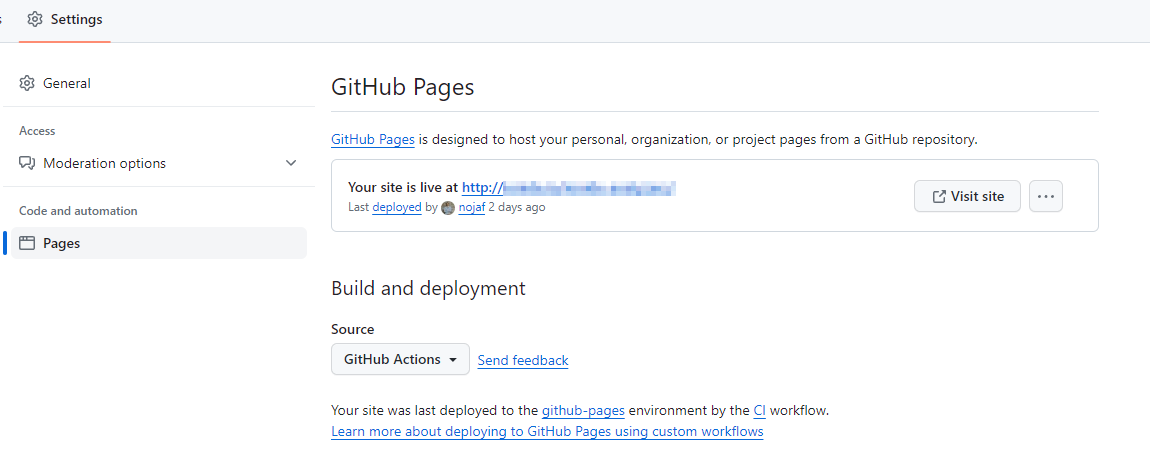
\includegraphics[width=1.0\textwidth]{./content/img/github-pages-settings.png}
\caption{Enable deploy from Actions}
\end{figure}



The typical flow is to publish your documentation after a release or after new commits were added to the default branch.

Let's create a very basic Action that will deploy our website after pushing to main:


Create a file \texttt{.github/workflows/docs.yml}:
\begin{lstlisting}
name: Docs

# Trigger this Action when new code is pushed to the main branch
on:
  push:
    branches:
      - main

# We need some permissions to publish to Github Pages
permissions:
  contents: write
  pages: write
  id-token: write

jobs:
  build:
    runs-on: ubuntu-latest
    steps:
      # Checkout the source code
      - uses: actions/checkout@v4
      # Setup dotnet, please use a global.json to ensure the right SDK is used!
      - name: Setup .NET
        uses: actions/setup-dotnet@v3
      # Restore the local tools
      - name: Restore tools
        run: dotnet tool restore
      # Build the code for the API documentation
      - name: Build code
        run: dotnet build -c Release YourSolution.sln
      # Generate the documentation files
      - name: Generate the documentation'
        run: dotnet fsdocs build --properties Configuration=Release
      # Upload the static files
      - name: Upload documentation
        uses: actions/upload-pages-artifact@v2
        with:
          path: ./output
  
  # GitHub Actions recommends deploying in a separate job.
  deploy:
    runs-on: ubuntu-latest
    needs: build
    steps:
      - name: Deploy to GitHub Pages
        id: deployment
        uses: actions/deploy-pages@v2

\end{lstlisting}


⚠️ Careful yaml is indentation sensitive!
\subsection*{Next steps}



Mission accomplished, right? If everything went well, you should have a published website at this point!

Here are some next steps you could consider:
\subsubsection*{Use fsx file in your documentation}



Create documentation using \href{../literate.html}{Literate Scripts}. A typical flow here is that you load your locate project binary into a script and create examples using the latest code:
\begin{lstlisting}[numbers=left]

[escapeinside=\\\{\}]
\prep{\#r} \str{"../src/Project1/bin/Debug/net6.0/Project1.dll"}

\kwd{open} \id{Project1}

\com{// Actual consumption of your project!}
\kwd{let} \id{result} \ops{=} \id{SomeType}{.}\id{SomeMethod}{(}\str{"foo"}{)}


\end{lstlisting}



When using the \texttt{--strict} flag in \texttt{dotnet fsdocs build}, your documentation generation will fail if your script contains errors.

This is useful to ensure your documentation is always in sync with your latest public API!
\subsubsection*{Automatically update to newer versions of fsdocs-tool}



Using \href{https://docs.github.com/en/code-security/dependabot/dependabot-version-updates/about-dependabot-version-updates}{Dependabot} you can easily receive new PR's with updates to your \texttt{dotnet} dependencies.


Create a \texttt{.github/dependabot.yml} file with:
\begin{lstlisting}
version: 2
updates:
  # Update to newer version of GitHub Actions
  - package-ecosystem: "github-actions"
    directory: "/"
    schedule:
      interval: "weekly"

  # Update to newer NuGet dependencies
  - package-ecosystem: "nuget"
    directory: "/"
    schedule:
      interval: "daily"

\end{lstlisting}


This will automatically create a new PR when there is an update to the \texttt{fsdocs} tool.


⚠️ P️lease be very careful, if you have followed along, we don't have any GitHub Actions right now that run against pull requests!

It is recommended to have an Action that builds your documentation against any incoming changes.

You typically want to lint code, run unit tests and perform other useful checks as well!


Example Action, \texttt{.github/workflows/ci.yml}:
\begin{lstlisting}
name: CI

on: [pull_request]

jobs:
  build:
    runs-on: ubuntu-latest

    steps:
    - uses: actions/checkout@v3
    - name: Setup .NET Core
      uses: actions/setup-dotnet@v3
    - name: Restore tools
      run: dotnet tool restore
    - name: Build
      run: dotnet build YourSolution.sln
    - name: Documentation
      run: dotnet fsdocs build

\end{lstlisting}


⚠️ Also never trust any update to \texttt{fsdocs} blindly, always check the \href{https://github.com/fsprojects/FSharp.Formatting/blob/main/RELEASE\_NOTES.md}{release notes} to see if there are any breaking changes.


\end{document}